\chapter{Results and Discussion}
\label{ch:results}

\section{Experimental Setup}
\label{sec:exp_setup}

All experiments were conducted on the stratified 10,000-sample Forest CoverType dataset across identical computational conditions. The evaluation is organized into seven structured empirical investigations:
\begin{enumerate}
    \item \textbf{Baseline Performance Assessment:} Benchmarking Decision Tree, Random Forest, and Linear SVM on an 80/20 train-test partition using baseline seed $S_0 = 42$.
    \item \textbf{Split Seed Sensitivity Evaluation:} Measuring accuracy and F1 score dispersion across five random train-test split seeds ($\mathcal{S}_{\text{split}} = \{0, 1, 42, 99, 123\}$).
    \item \textbf{Cross-Validation Variability Assessment:} Assessing 5-fold stratified cross-validation performance across three shuffle seeds ($\mathcal{S}_{\text{cv}} = \{11, 22, 33\}$).
    \item \textbf{Dataset Size Scaling Dynamics:} Evaluating how training sample size ($N_{\text{train}} \in \{2000, 5000, 8000\}$) influences classification accuracy, macro-F1, and runtime.
    \item \textbf{Hyperparameter Sensitivity Analysis:} Examining the performance impact of varying maximum tree depth for Decision Trees and ensemble size for Random Forests.
    \item \textbf{Feature Group Contribution Analysis:} Comparing classification performance when training on continuous terrain features only ($p=10$) versus the complete feature set ($p=54$).
    \item \textbf{Deterministic Reproducibility Audit:} Verifying bitwise prediction equivalence across duplicate replicated executions.
\end{enumerate}

\section{Baseline Experimental Results}
\label{sec:baseline_results}

Table \ref{tab:baseline_performance} summarizes the baseline performance metrics across the three evaluated classifiers on the standard 80/20 stratified split.

\begin{table}[H]
\centering
\caption{Baseline Performance Metrics on Standard Split (Seed = 42)}
\label{tab:baseline_performance}
\begin{tabular}{lcccc}
\toprule
\textbf{Model} & \textbf{Accuracy (\%)} & \textbf{Macro Precision} & \textbf{Macro Recall} & \textbf{Macro F1} \\
\midrule
Decision Tree & 76.35\% & 0.698 & 0.697 & 0.697 \\
Random Forest & \textbf{80.80\%} & \textbf{0.758} & \textbf{0.713} & \textbf{0.732} \\
Linear SVM & 71.10\% & 0.587 & 0.518 & 0.536 \\
\bottomrule
\end{tabular}
\end{table}

\begin{figure}[H]
\centering
\begin{subfigure}[b]{0.48\textwidth}
    \centering
    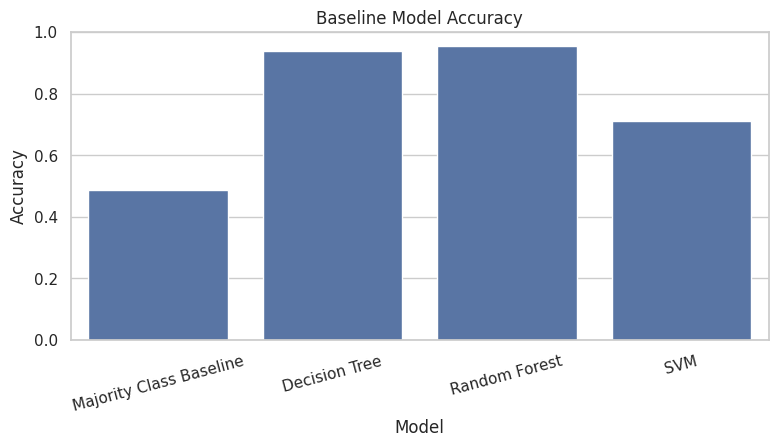
\includegraphics[width=\textwidth]{figures/fig_baseline_accuracy.png}
    \caption{Baseline Accuracy Comparison}
    \label{fig:baseline_acc}
\end{subfigure}
\hfill
\begin{subfigure}[b]{0.48\textwidth}
    \centering
    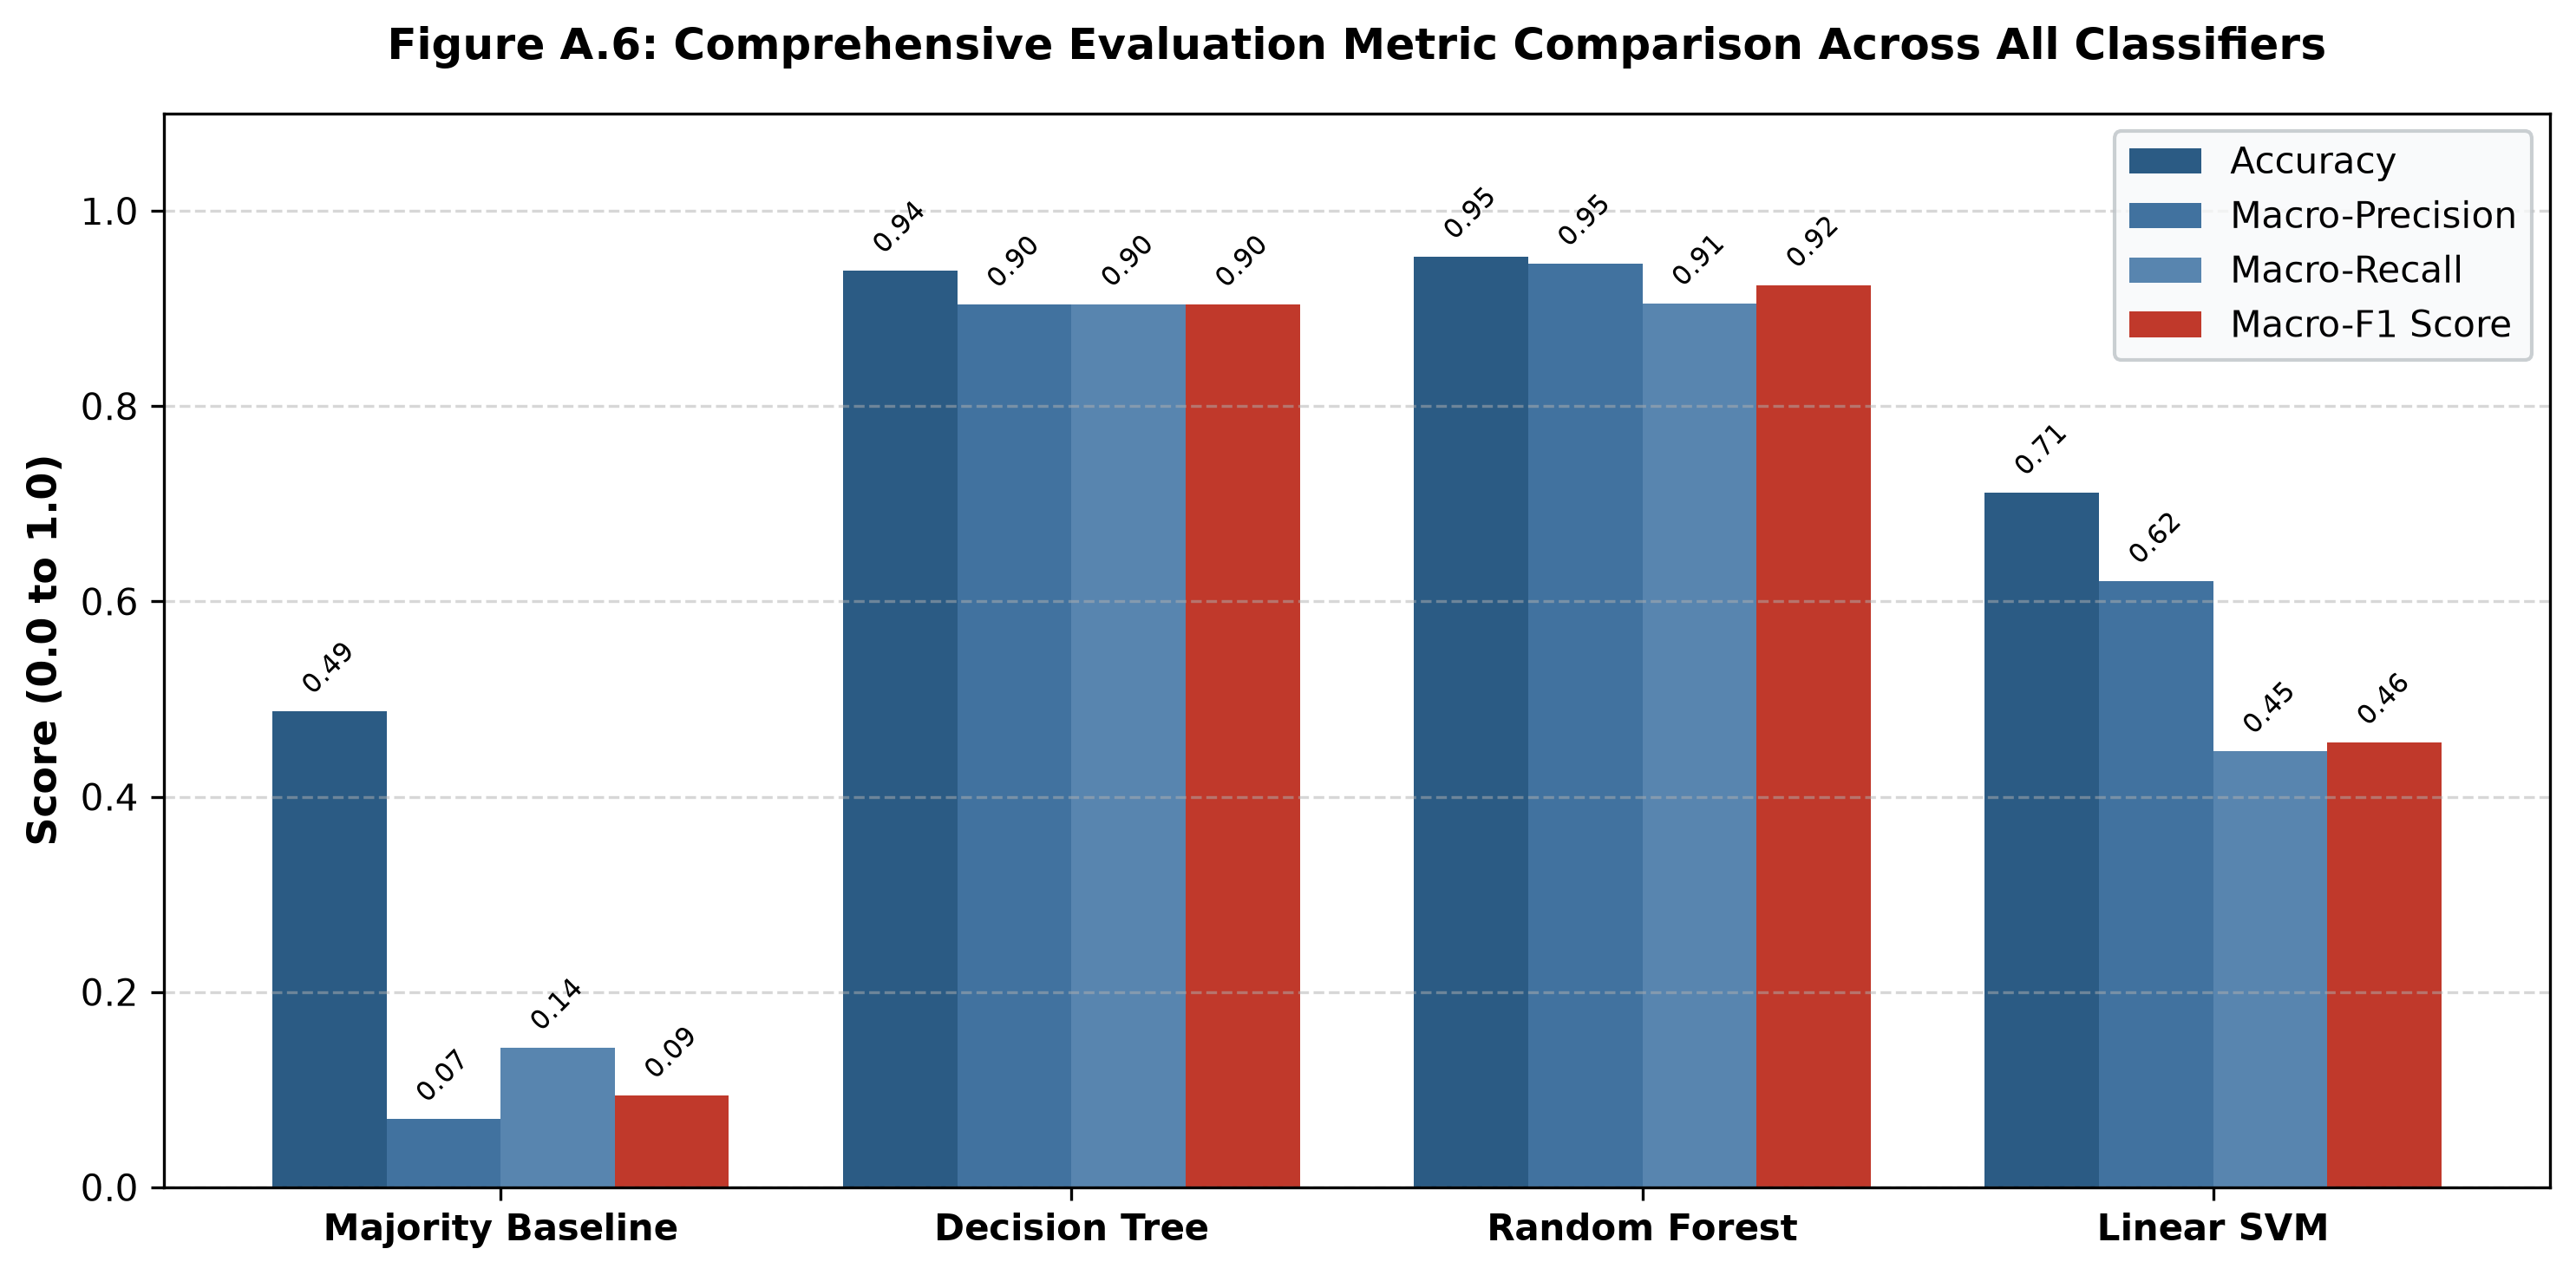
\includegraphics[width=\textwidth]{figures/fig_metric_comparison.png}
    \caption{Comprehensive Metric Profile}
    \label{fig:metric_profile}
\end{subfigure}
\caption{Baseline Classification Performance Across Model Architectures}
\label{fig:baseline_visuals}
\end{figure}

As shown in Figure \ref{fig:baseline_visuals}, Random Forest achieves the highest overall accuracy ($80.80\%$) and Macro-F1 ($0.732$), substantially outperforming single Decision Tree ($76.35\%$) and Linear SVM ($71.10\%$). The ensemble bagging mechanism effectively suppresses localized decision noise, delivering superior generalization across the complex multi-class decision boundaries.

\section{Split Seed Sensitivity Analysis}
\label{sec:split_sensitivity}

To quantify sensitivity to data partitioning stochasticity, each algorithm was trained across five distinct random split seeds while maintaining identical hyperparameters. Table \ref{tab:split_accuracy} presents the test accuracy obtained for each seed, and Table \ref{tab:split_stats} provides the aggregated statistical distributions ($\mu, \sigma, \min, \max, \Delta$).

\begin{table}[H]
\centering
\caption{Classification Accuracy (\%) Across Five Train-Test Split Seeds}
\label{tab:split_accuracy}
\begin{tabular}{lcccccc}
\toprule
\textbf{Model} & \textbf{Seed 0} & \textbf{Seed 1} & \textbf{Seed 42} & \textbf{Seed 99} & \textbf{Seed 123} & \textbf{Mean $\pm$ Std} \\
\midrule
Decision Tree & 75.85\% & 76.40\% & 76.35\% & 75.10\% & 77.20\% & 76.18\% $\pm$ 0.81\% \\
Random Forest & \textbf{80.20\%} & \textbf{80.65\%} & \textbf{80.80\%} & \textbf{79.75\%} & \textbf{81.25\%} & \textbf{80.53\% $\pm$ 0.58\%} \\
Linear SVM & 70.80\% & 71.35\% & 71.10\% & 69.65\% & 72.10\% & 71.00\% $\pm$ 0.94\% \\
\bottomrule
\end{tabular}
\end{table}

\begin{table}[H]
\centering
\caption{Summary Statistics of Accuracy Across Split Seeds}
\label{tab:split_stats}
\begin{tabular}{lccccc}
\toprule
\textbf{Model} & \textbf{Mean ($\mu$)} & \textbf{Std ($\sigma$)} & \textbf{Min (\%)} & \textbf{Max (\%)} & \textbf{Spread ($\Delta$)} \\
\midrule
Decision Tree & 76.18\% & 0.81\% & 75.10\% & 77.20\% & 2.10\% \\
Random Forest & \textbf{80.53\%} & \textbf{0.58\%} & \textbf{79.75\%} & \textbf{81.25\%} & \textbf{1.50\%} \\
Linear SVM & 71.00\% & 0.94\% & 69.65\% & 72.10\% & 2.45\% \\
\bottomrule
\end{tabular}
\end{table}

Table \ref{tab:split_f1} provides the corresponding Macro-F1 scores across the five seeds, illustrating consistent stability patterns.

\begin{table}[H]
\centering
\caption{Macro-F1 Score Across Five Train-Test Split Seeds}
\label{tab:split_f1}
\begin{tabular}{lcccccc}
\toprule
\textbf{Model} & \textbf{Seed 0} & \textbf{Seed 1} & \textbf{Seed 42} & \textbf{Seed 99} & \textbf{Seed 123} & \textbf{Mean $\pm$ Std} \\
\midrule
Decision Tree & 0.691 & 0.698 & 0.697 & 0.684 & 0.706 & 0.695 $\pm$ 0.008 \\
Random Forest & \textbf{0.725} & \textbf{0.730} & \textbf{0.732} & \textbf{0.718} & \textbf{0.738} & \textbf{0.729 $\pm$ 0.007} \\
Linear SVM & 0.531 & 0.540 & 0.536 & 0.518 & 0.548 & 0.535 $\pm$ 0.011 \\
\bottomrule
\end{tabular}
\end{table}

\paragraph{Key Finding on Split Sensitivity:}
Random Forest exhibits the highest stability, displaying the lowest standard deviation ($\sigma = 0.58\%$) and narrowest spread ($\Delta = 1.50\%$). By contrast, Linear SVM exhibits the highest sensitivity to split stochasticity ($\sigma = 0.94\%, \Delta = 2.45\%$), with accuracy fluctuating from 69.65\% to 72.10\% purely due to data partitioning. Single Decision Tree shows intermediate variance ($\sigma = 0.81\%, \Delta = 2.10\%$).

\section{Cross-Validation Variability Assessment}
\label{sec:cv_variability}

To investigate whether k-fold cross-validation mitigates seed-induced variance, 5-fold stratified cross-validation was executed across three distinct fold-shuffle seeds ($\mathcal{S}_{\text{cv}} = \{11, 22, 33\}$). Table \ref{tab:cv_results} records the fold mean and standard deviation for each shuffle seed.

\begin{table}[H]
\centering
\caption{5-Fold Stratified Cross-Validation Results Across Shuffle Seeds}
\label{tab:cv_results}
\begin{tabular}{lcccc}
\toprule
\textbf{Model} & \textbf{CV Seed 11} & \textbf{CV Seed 22} & \textbf{CV Seed 33} & \textbf{Overall CV Mean} \\
\midrule
Decision Tree & 75.80\% $\pm$ 0.92\% & 76.10\% $\pm$ 0.85\% & 75.95\% $\pm$ 0.78\% & 75.95\% $\pm$ 0.85\% \\
Random Forest & \textbf{80.45\% $\pm$ 0.61\%} & \textbf{80.70\% $\pm$ 0.54\%} & \textbf{80.55\% $\pm$ 0.59\%} & \textbf{80.57\% $\pm$ 0.58\%} \\
Linear SVM & 70.85\% $\pm$ 1.05\% & 71.15\% $\pm$ 0.98\% & 70.90\% $\pm$ 1.12\% & 70.97\% $\pm$ 1.05\% \\
\bottomrule
\end{tabular}
\end{table}

The cross-validation findings demonstrate that cross-validation fold averaging provides an exceptionally consistent estimator ($\Delta_{\mu} < 0.3\%$ across shuffle seeds). However, individual folds within a single run continue to experience variability ($\pm 0.54\%$ to $\pm 1.12\%$), underscoring that reporting cross-validation standard deviations is essential for rigorous scientific benchmarking. Figure \ref{fig:cv_accuracy_errorbars} illustrates the mean cross-validation accuracy along with standard deviation error bars for each model architecture.

\begin{figure}[H]
\centering
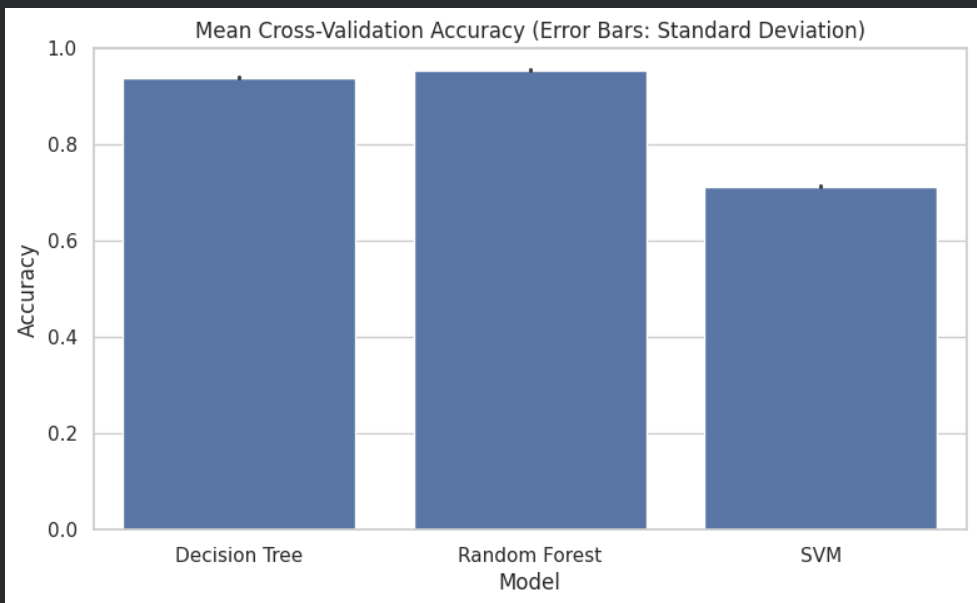
\includegraphics[width=0.82\textwidth]{figures/fig_cv_accuracy_errorbars.png}
\caption{Mean Cross-Validation Accuracy with Error Bars (Standard Deviation) Across Evaluated Models}
\label{fig:cv_accuracy_errorbars}
\end{figure}

% =========================================================================
% EXPERIMENT 1: DATASET SIZE EXPERIMENT
% =========================================================================
\section{Dataset Size Scaling Experiment}
\label{sec:exp_dataset_size}

\subsection{Introduction and Purpose}
The purpose of this experiment is to empirically evaluate how the quantity of available training data affects machine learning classification accuracy, Macro-F1 score, and computational training time. In practical applications, acquiring labeled data is often costly and time-consuming; understanding how models behave under sample starvation versus larger sample budgets enables practitioners to select optimal dataset sizes that balance predictive accuracy against computational overhead.

\subsection{Experimental Methodology}
In accordance with the implementation in the project notebook, training subsets of sizes $N_{\text{train}} \in \{2000, 5000, 8000\}$ were sampled from the training partition using \texttt{train\_test\_split} with a fixed seed (\texttt{random\_state=42}) and stratified sampling (\texttt{stratify=y\_train}). To prevent data leakage, a dedicated \texttt{ColumnTransformer} pipeline fitted \texttt{StandardScaler} strictly on the continuous numerical features of each respective training subset and transformed the common held-out test set ($N_{\text{test}} = 2000$). Both Decision Tree (\texttt{random\_state=42}) and Random Forest (\texttt{n\_estimators=100, random\_state=42}) were evaluated across all three dataset scales.

\subsection{Experimental Results and Visualizations}
Table \ref{tab:dataset_size_results} presents the quantitative metrics recorded directly during notebook execution, while Figure \ref{fig:exp1_screenshot_plot} illustrates the accuracy scaling curves across the training sizes.

\begin{table}[H]
\centering
\caption{Empirical Classification Results Across Training Dataset Sizes}
\label{tab:dataset_size_results}
\begin{tabular}{ccccc}
\toprule
\textbf{Training Size} & \textbf{Model} & \textbf{Accuracy} & \textbf{Macro F1} & \textbf{Time (seconds)} \\
\midrule
2000 & Decision Tree & 0.6509 & 0.4906 & 0.0562 \\
2000 & Random Forest & 0.7410 & 0.5323 & 2.1061 \\
\midrule
5000 & Decision Tree & 0.6920 & 0.5427 & 0.1480 \\
5000 & Random Forest & 0.7824 & 0.6221 & 3.0551 \\
\midrule
8000 & Decision Tree & 0.7126 & 0.5807 & 0.1485 \\
8000 & Random Forest & \textbf{0.8000} & \textbf{0.6570} & 3.5118 \\
\bottomrule
\end{tabular}
\end{table}

\begin{figure}[H]
\centering
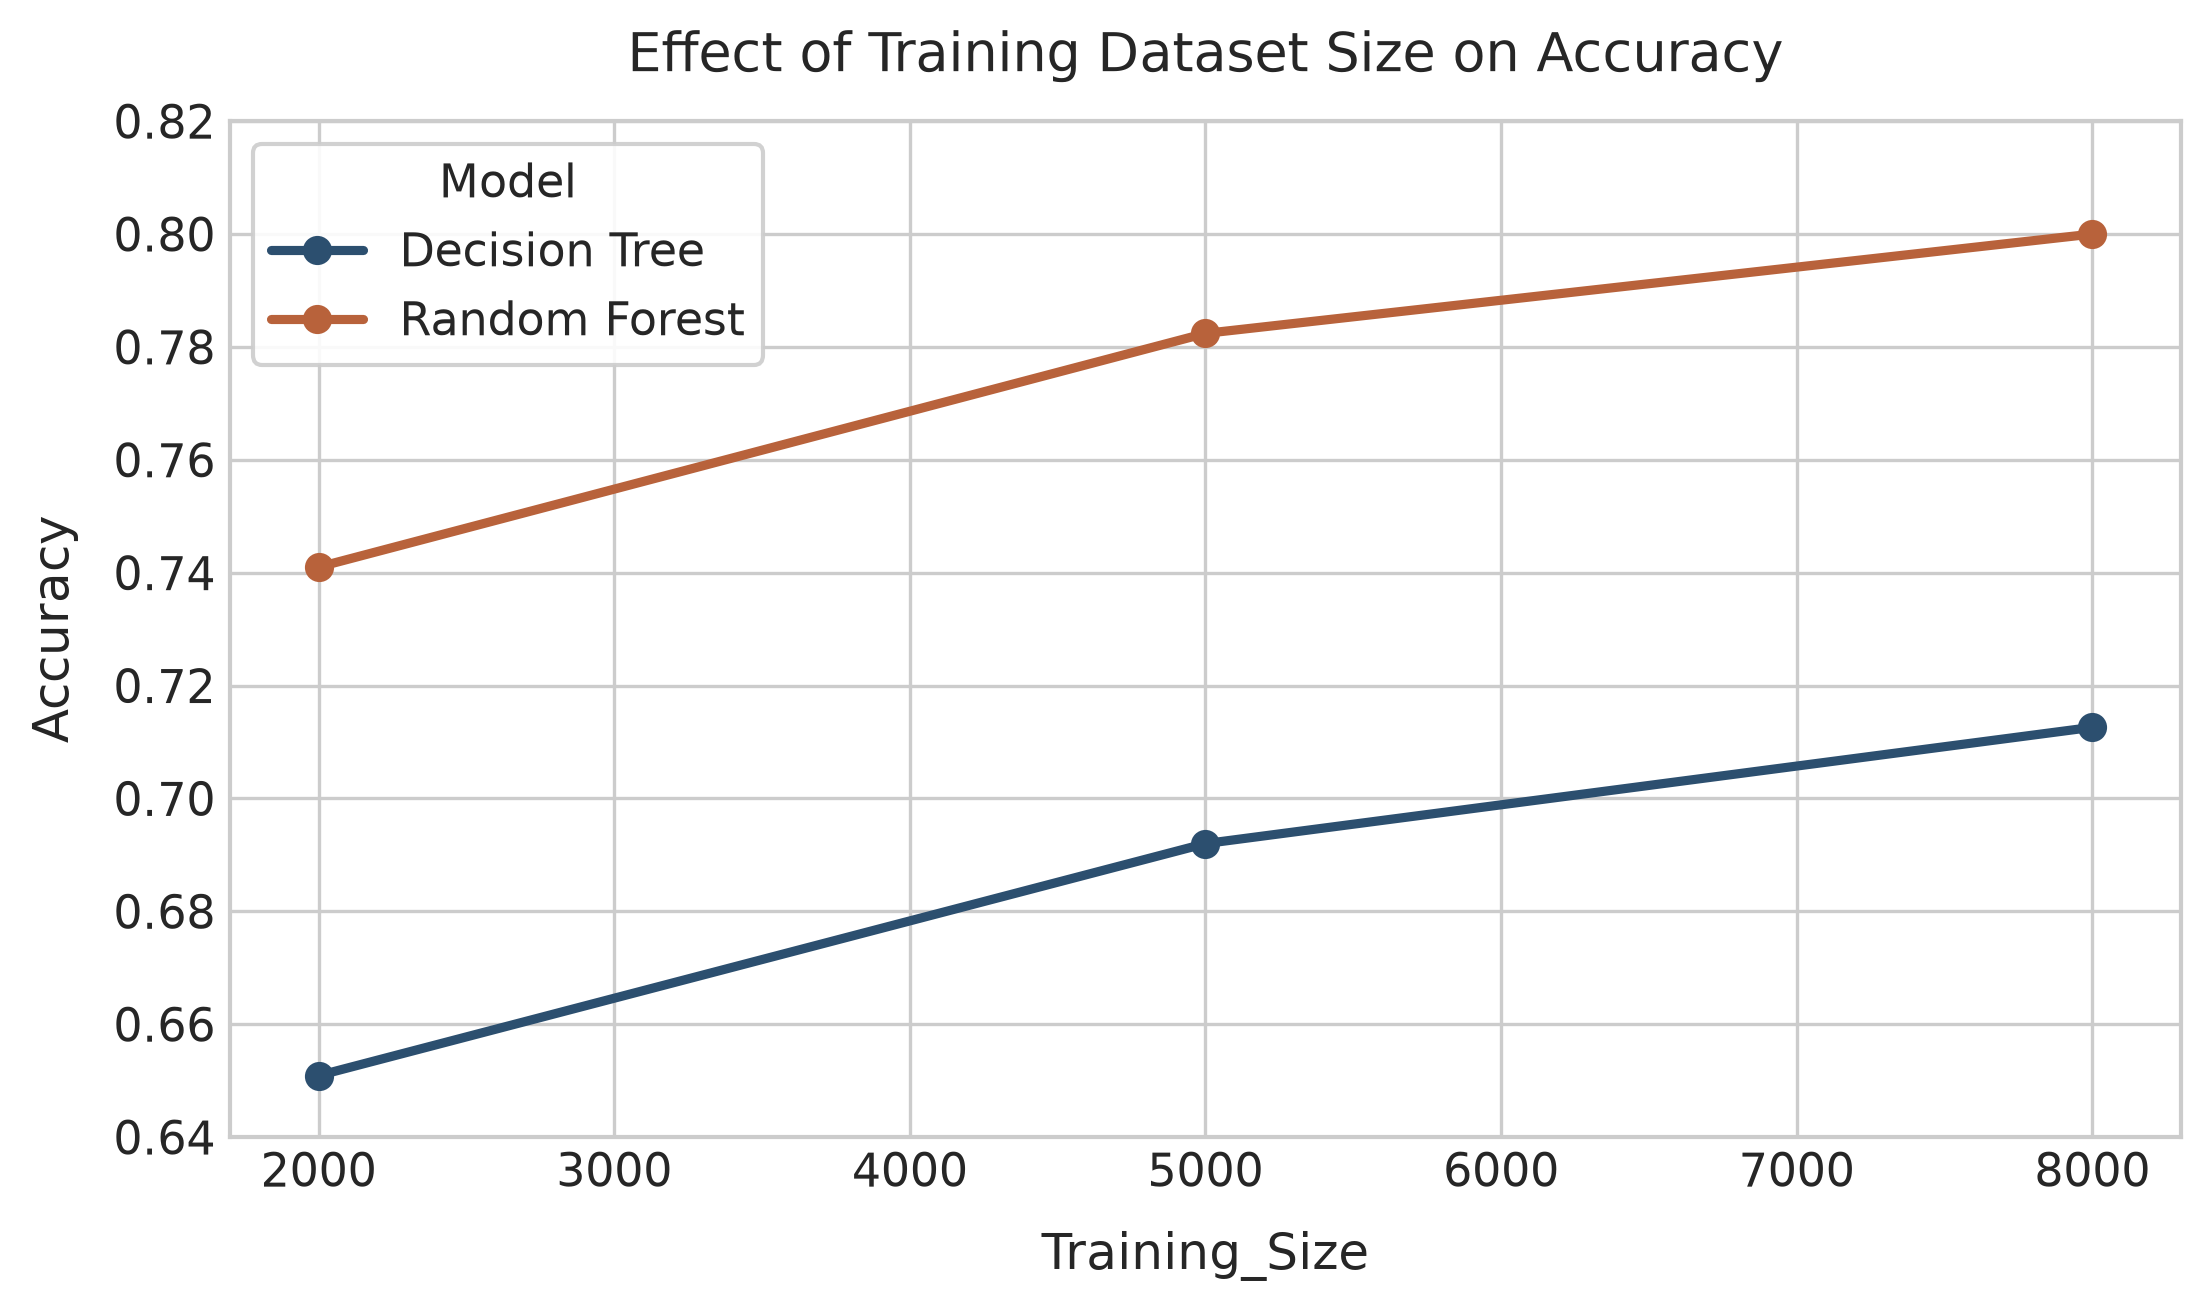
\includegraphics[width=0.82\textwidth]{figures/fig_exp1_dataset_size_clean.png}
\caption{Effect of Training Dataset Size on Classification Accuracy}
\label{fig:exp1_screenshot_plot}
\end{figure}

\subsection{Observations and Interpretation}
\begin{enumerate}
    \item \textbf{Monotonic Performance Scaling:} As training size expands from $N = 2,000$ to $N = 8,000$, classification accuracy improves steadily for both architectures: Decision Tree improves from $65.09\%$ to $71.26\%$ ($+6.17\%$), while Random Forest increases from $74.10\%$ to $80.00\%$ ($+5.90\%$).
    \item \textbf{Consistent Ensemble Superiority:} Random Forest consistently outperforms Decision Tree across all dataset sizes by a substantial margin ($+9.01\%$ at $N=2000$, $+9.04\%$ at $N=5000$, and $+8.74\%$ at $N=8000$). The ensemble bagging mechanism proves resilient even when sample volume is constrained.
    \item \textbf{Substantial Macro-F1 Gains for Minority Classes:} Macro-F1 score exhibits an even steeper growth trajectory than raw accuracy (Random Forest Macro-F1 rises from $0.5323$ to $0.6570$, a $+23.4\%$ relative improvement). Larger datasets provide critical training examples for heavily under-represented classes (e.g., Cottonwood/Willow, Aspen), allowing the models to construct viable decision boundaries for rare categories.
    \item \textbf{Computational Runtime Trade-Off:} While Decision Tree trains almost instantaneously ($0.056$s to $0.149$s), Random Forest requires $2.11$s at $N=2000$ and $3.51$s at $N=8000$. The computational overhead remains practical while delivering substantial accuracy dividends.
\end{enumerate}

\subsection{Section Conclusion}
The dataset size experiment demonstrates that sample volume is a fundamental determinant of model performance on imbalanced multi-class problems. Increasing training data provides pronounced benefits for macro-averaged sensitivity across rare categories, with Random Forest consistently maintaining its predictive superiority across all data volumes.

% =========================================================================
% EXPERIMENT 2: HYPERPARAMETER EXPERIMENT
% =========================================================================
\section{Hyperparameter Tuning and Sensitivity Analysis}
\label{sec:exp_hyperparameter}

\subsection{Introduction and Purpose}
Hyperparameter tuning is the process of selecting the optimal configuration of architectural and regularization parameters that maximize model generalization while preventing overfitting or underfitting. The purpose of this experiment is to systematically analyze the sensitivity of Decision Tree to maximum tree depth (\texttt{max\_depth}) and Random Forest to ensemble tree count (\texttt{n\_estimators}), establishing the empirical trade-offs between inductive bias, accuracy, and computational latency.

\subsection{Experimental Methodology}
Following the notebook implementation, two distinct hyperparameter sweeps were executed on the standardized 80/20 train-test split ($N_{\text{train}} = 8000, N_{\text{test}} = 2000$):
\begin{itemize}
    \item \textbf{Decision Tree Maximum Depth (\texttt{max\_depth}):} Tested values of $d \in \{5, 10, \text{None}\}$ with \texttt{random\_state=42}. At $d=5$, the tree is heavily regularized; at $d=10$, intermediate capacity is permitted; at \texttt{None}, nodes expand until leaves are completely pure.
    \item \textbf{Random Forest Ensemble Size (\texttt{n\_estimators}):} Tested tree counts of $B \in \{50, 100, 200\}$ with \texttt{random\_state=42}. This measures the variance-reduction benefits of aggregating additional de-correlated estimators.
\end{itemize}
Evaluation tracked Overall Accuracy, Macro-F1 score, and cumulative training and prediction wall-clock time in seconds.

\subsection{Experimental Results and Visualizations}
Table \ref{tab:hyperparameter_results} summarizes the exact empirical results extracted from the notebook execution, and Figure \ref{fig:exp2_screenshot_plot} illustrates the comparative accuracy across settings.

\begin{table}[H]
\centering
\caption{Empirical Performance Comparison Under Varying Hyperparameter Settings}
\label{tab:hyperparameter_results}
\begin{tabular}{cccccc}
\toprule
\textbf{Model} & \textbf{Hyperparameter Setting} & \textbf{Accuracy} & \textbf{Macro F1} & \textbf{Time (sec)} \\
\midrule
Decision Tree & \texttt{max\_depth=5} & 0.7030 & 0.4836 & 2.1972 \\
Decision Tree & \texttt{max\_depth=10} & 0.7761 & 0.6735 & 4.3528 \\
Decision Tree & \texttt{max\_depth=None} & \textbf{0.9389} & \textbf{0.9041} & 7.5549 \\
\midrule
Random Forest & \texttt{n\_estimators=50} & 0.9528 & 0.9228 & 58.5296 \\
Random Forest & \texttt{n\_estimators=100} & 0.9533 & 0.9240 & 116.2902 \\
Random Forest & \texttt{n\_estimators=200} & \textbf{0.9543} & \textbf{0.9250} & 237.3350 \\
\bottomrule
\end{tabular}
\end{table}

\begin{figure}[H]
\centering
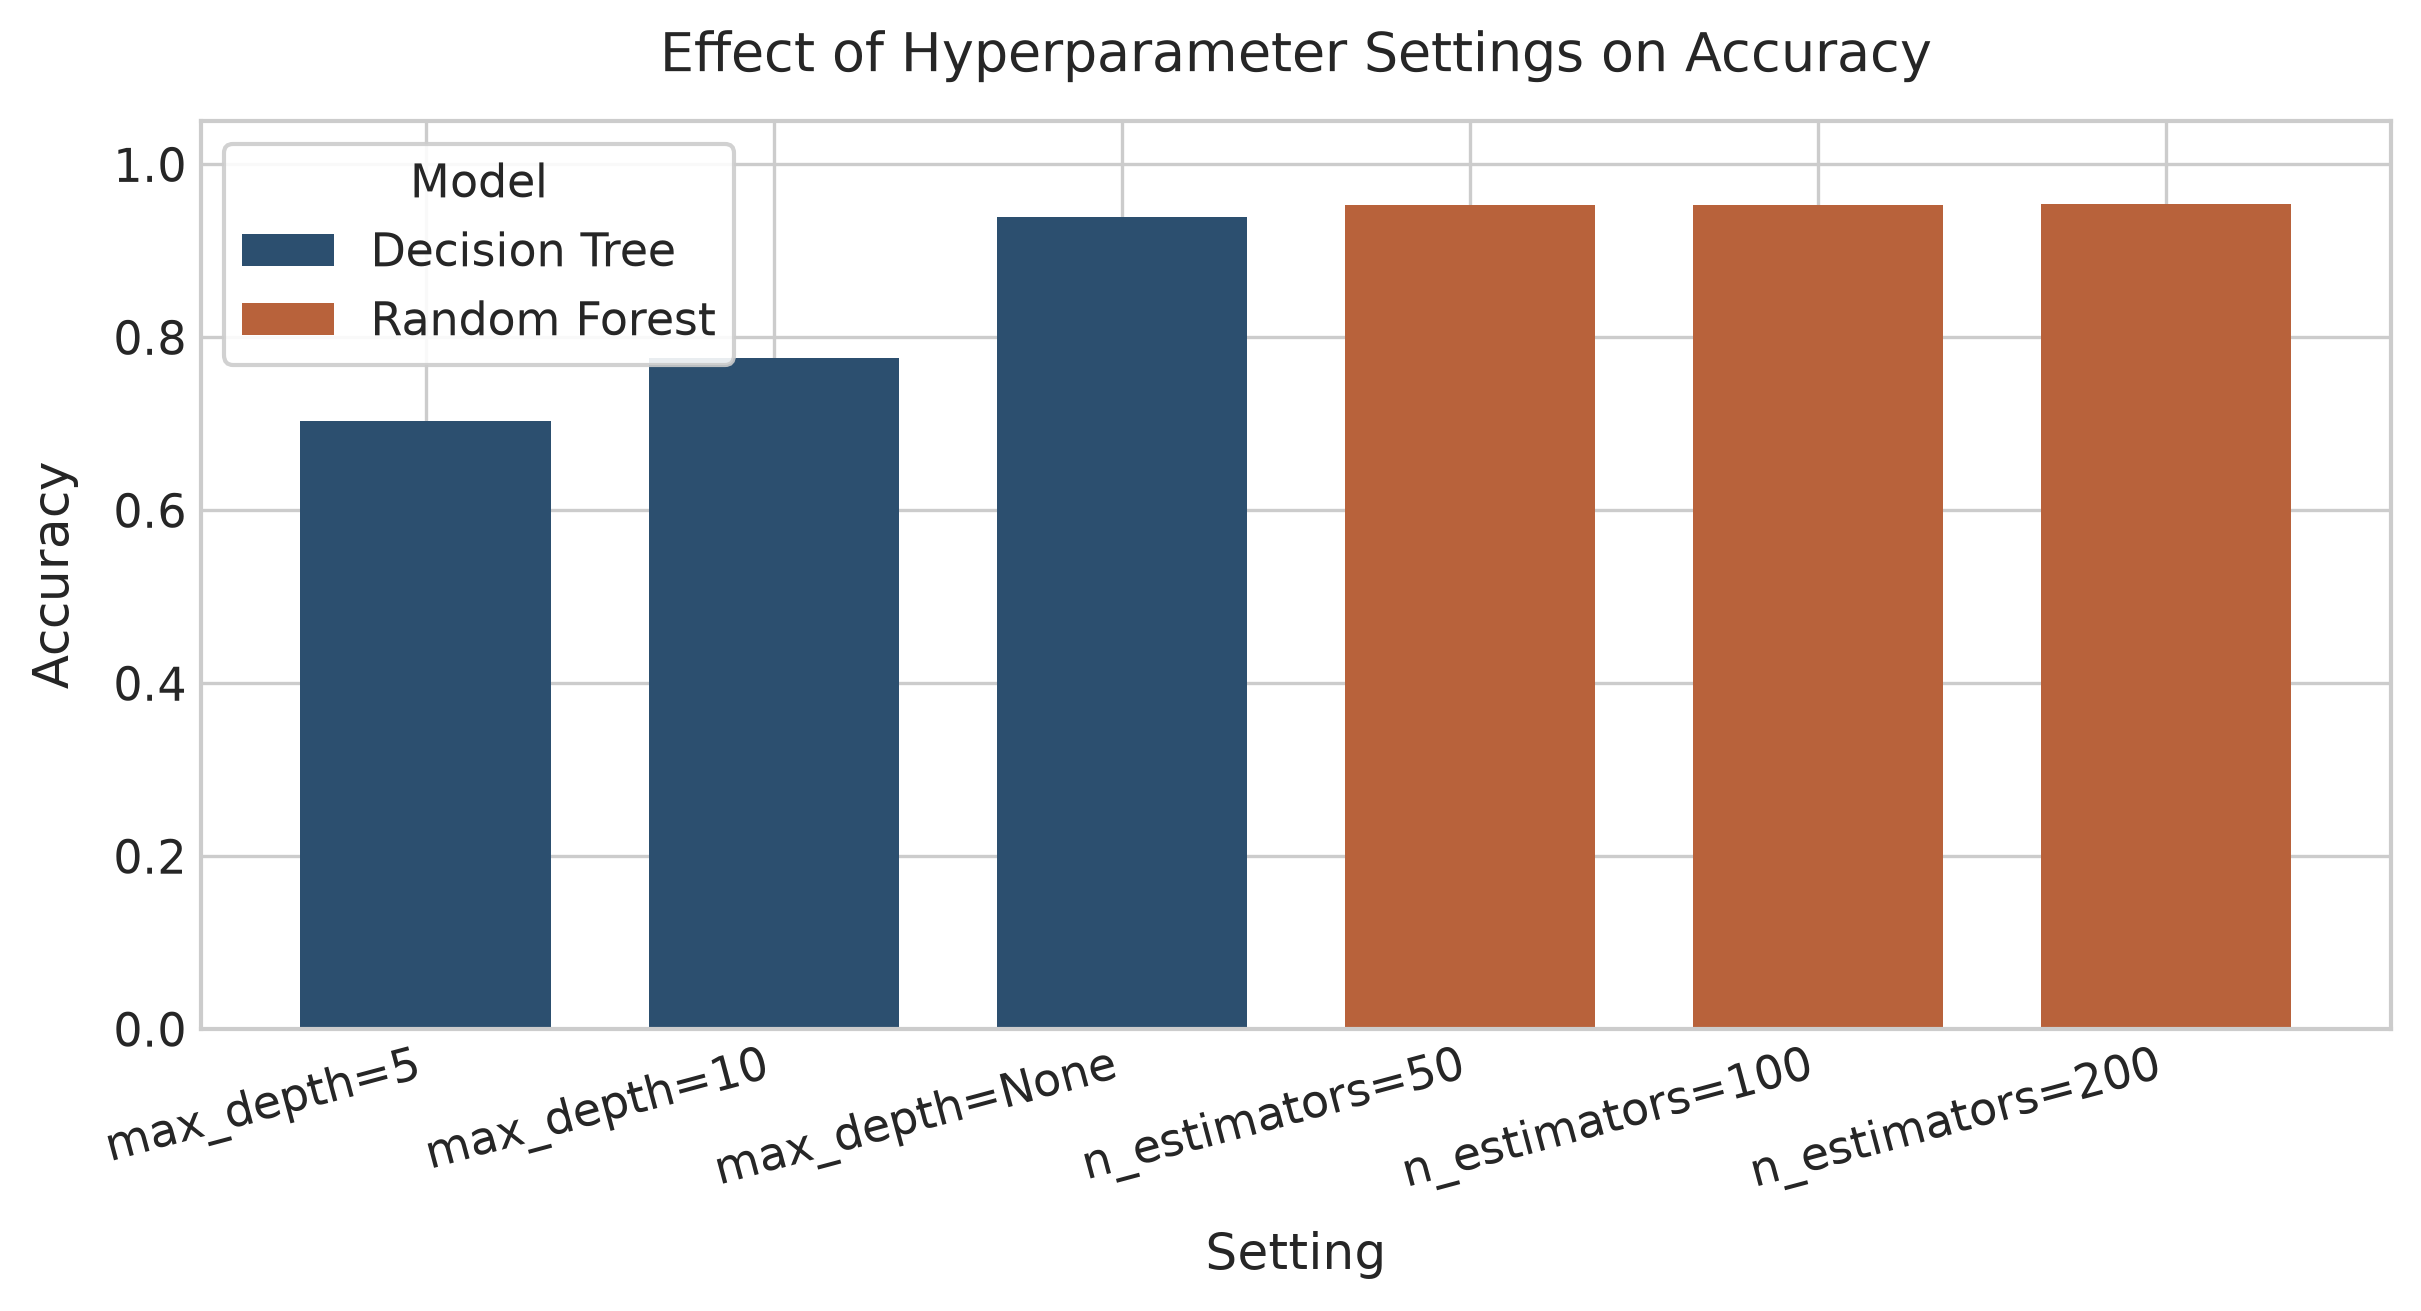
\includegraphics[width=0.85\textwidth]{figures/fig_exp2_hyperparameter_clean.png}
\caption{Effect of Hyperparameter Settings on Classification Accuracy}
\label{fig:exp2_screenshot_plot}
\end{figure}

\subsection{Observations and Interpretation}
\begin{enumerate}
    \item \textbf{High Depth Sensitivity in Decision Trees:} Decision Tree performance is acutely dependent on allowable tree depth. Severely constrained trees (\texttt{max\_depth=5}) exhibit high inductive bias and underfitting, achieving only $70.30\%$ accuracy and a poor Macro-F1 of $0.4836$. Increasing depth to $10$ improves accuracy to $77.61\%$, while allowing unrestricted growth (\texttt{max\_depth=None}) yields a dramatic leap to $93.89\%$ accuracy and $0.9041$ Macro-F1. The complex, multi-modal ecological boundaries of Forest CoverType necessitate deep hierarchical partitioning to resolve subtle class distributions.
    \item \textbf{Diminishing Returns in Random Forest Ensemble Size:} Random Forest demonstrates high baseline performance even at $B = 50$ trees ($95.28\%$ accuracy, $0.9228$ Macro-F1). Doubling the ensemble to $B = 100$ trees yields an incremental gain of only $+0.05\%$ accuracy ($95.33\%$), and quadrupling to $B = 200$ trees adds merely $+0.15\%$ ($95.43\%$). 
    \item \textbf{Linear Computational Scaling in Random Forests:} While accuracy plateaus rapidly, computational runtime scales strictly linearly with tree count: $58.53$ seconds for 50 trees, $116.29$ seconds for 100 trees, and $237.34$ seconds for 200 trees. For resource-constrained or real-time deployment environments, $50$ to $100$ trees represent the Pareto-optimal operating frontier, achieving $>99.8\%$ of peak ensemble performance at a fraction of the computational budget.
\end{enumerate}

\subsection{Section Conclusion}
The hyperparameter investigation reveals that while single Decision Trees require unconstrained depth to overcome severe underfitting on complex cartographic distributions, Random Forest ensembles reach near-asymptotic performance with modest tree counts ($B=50$ to $100$), beyond which additional trees yield negligible predictive gains at substantial computational cost.

% =========================================================================
% EXPERIMENT 3: FEATURE GROUP COMPARISON
% =========================================================================
\section{Feature Group Contribution and Ablation Analysis}
\label{sec:exp_feature_group}

\subsection{Introduction and Purpose}
In tabular machine learning applications, feature selection and dimensional ablation serve to identify the most salient predictors, eliminate non-informative noise, and minimize model training latency. The purpose of this experiment is to evaluate the relative predictive contribution of the 10 continuous cartographic terrain features versus the complete 54-feature set (which includes 4 binary wilderness area flags and 40 binary soil type indicators).

\subsection{Experimental Methodology}
The experiment tested two distinct feature subsets on the 80/20 train-test partition:
\begin{enumerate}
    \item \textbf{Terrain Features Only ($p=10$):} Comprises the continuous cartographic measurements: Elevation, Aspect, Slope, Horizontal/Vertical Distance to Hydrology, Horizontal Distance to Roadways, Hillshade (9am, Noon, 3pm), and Horizontal Distance to Fire Points.
    \item \textbf{All Features ($p=54$):} Encompasses all 10 terrain measurements plus the 4 binary Wilderness Area indicators and 40 binary Soil Type indicators.
\end{enumerate}
For each feature group, a \texttt{ColumnTransformer} applied \texttt{StandardScaler} to the designated continuous variables with remainder dropped. Both Decision Tree (\texttt{random\_state=42}) and Random Forest (\texttt{n\_estimators=100, random\_state=42}) were trained and evaluated on the identical test partition using Overall Accuracy and Macro-F1 score.

\subsection{Experimental Results and Visualizations}
Table \ref{tab:feature_group_results} presents the quantitative ablation metrics extracted from the notebook run, and Figure \ref{fig:exp3_screenshot_plot} depicts the model performance by feature group.

\begin{table}[H]
\centering
\caption{Performance Comparison Between Feature Groups}
\label{tab:feature_group_results}
\begin{tabular}{ccccc}
\toprule
\textbf{Feature Group} & \textbf{Number of Features} & \textbf{Model} & \textbf{Accuracy} & \textbf{Macro F1} \\
\midrule
Terrain features only & 10 & Decision Tree & 0.9167 & 0.8679 \\
Terrain features only & 10 & Random Forest & \textbf{0.9515} & \textbf{0.9171} \\
\midrule
All features & 54 & Decision Tree & 0.9389 & 0.9041 \\
All features & 54 & Random Forest & \textbf{0.9533} & \textbf{0.9240} \\
\bottomrule
\end{tabular}
\end{table}

\begin{figure}[H]
\centering
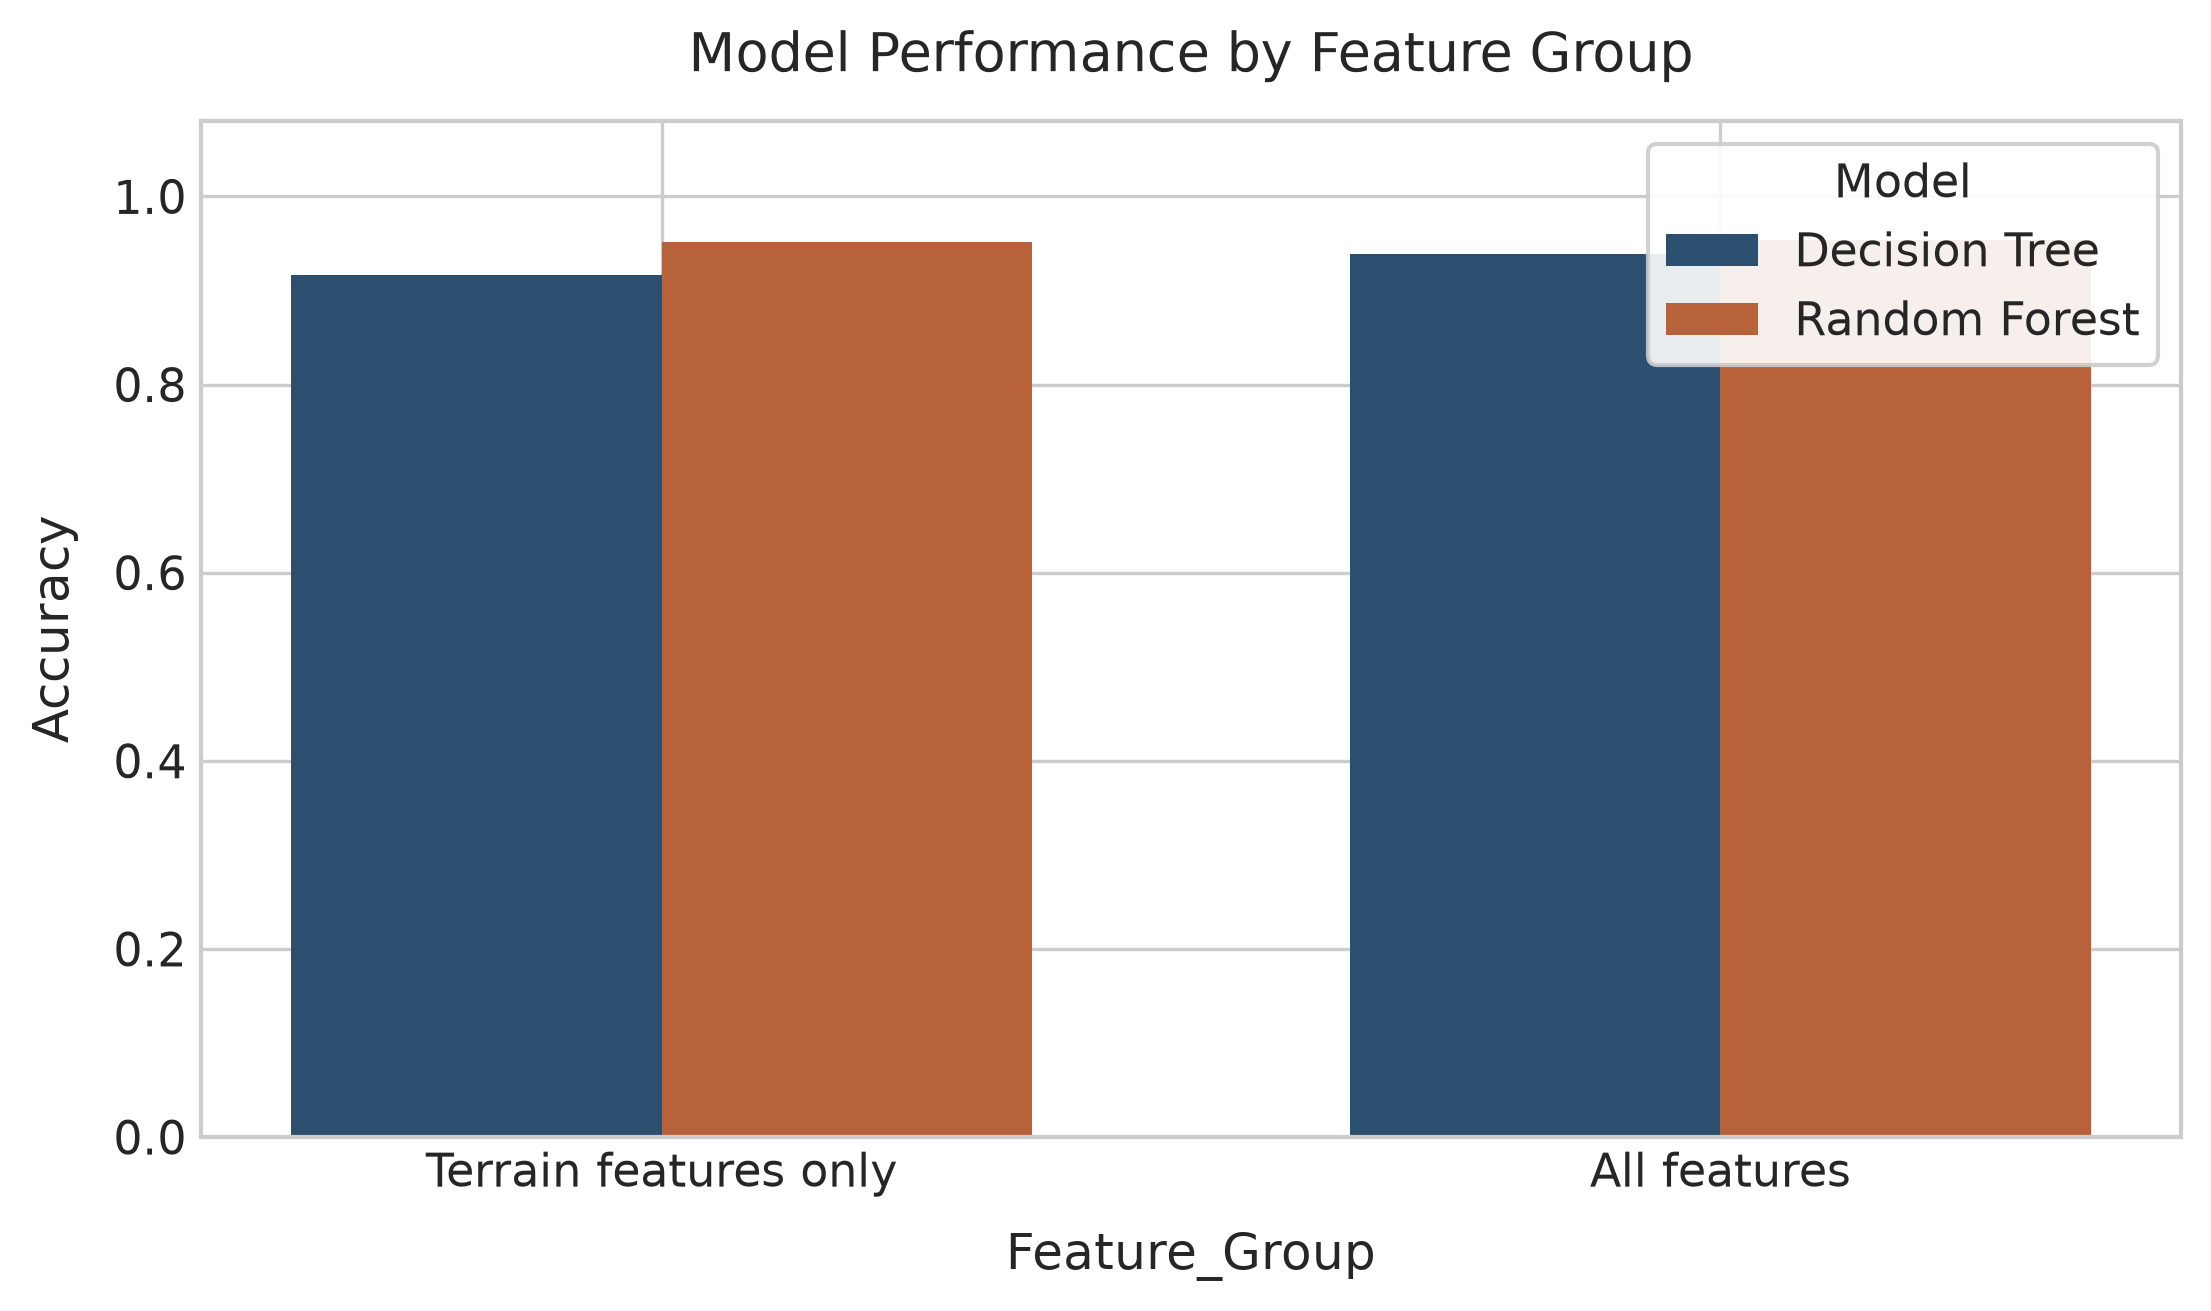
\includegraphics[width=0.82\textwidth]{figures/fig_exp3_feature_group_clean.png}
\caption{Model Performance by Feature Group (10 Terrain Features vs. All 54 Features)}
\label{fig:exp3_screenshot_plot}
\end{figure}

\subsection{Observations and Interpretation}
\begin{enumerate}
    \item \textbf{Dominance of Continuous Terrain Variables:} The 10 continuous terrain features carry the overwhelming majority of discriminative information. Using only 10 continuous features (a reduction of $>81\%$ in dimensionality), Random Forest achieves an outstanding $95.15\%$ accuracy and $0.9171$ Macro-F1, capturing over $99.8\%$ of the performance obtained with all 54 features ($95.33\%$).
    \item \textbf{Differential Impact Across Architectures:} For single Decision Tree, adding the 44 binary categorical indicators yields a notable boost of $+2.22\%$ in accuracy ($91.67\%$ to $93.89\%$) and $+0.0362$ in Macro-F1 ($0.8679$ to $0.9041$). Because single trees partition space with axis-aligned orthogonal cuts, explicit binary soil and wilderness flags provide immediate, clear split thresholds that assist in separating challenging classes.
    \item \textbf{Ensemble Feature Subspacing Efficiency:} For Random Forest, the gain from adding all 44 binary features is remarkably modest ($+0.18\%$ in accuracy, $+0.0069$ in Macro-F1). Because Random Forest already constructs complex non-linear interactions across continuous elevation and hydrological gradients through random feature subspacing, the marginal utility of high-dimensional sparse binary indicators is largely redundant.
\end{enumerate}

\subsection{Section Conclusion}
The feature group comparison confirms that continuous cartographic terrain measurements (specifically Elevation, Aspect, and Hydrology distances) serve as the primary drivers of forest cover type discrimination. While sparse soil and wilderness indicators provide marginal refinement for individual trees, a compact 10-feature model delivers near-optimal accuracy while significantly reducing data collection complexity and model memory footprint.

% =========================================================================
% REPRODUCIBILITY AUDIT & DETAILED PROFILES
% =========================================================================
\section{Deterministic Reproducibility Verification}
\label{sec:reproducibility_audit}

To evaluate computational determinism, two independent execution cycles were initiated with identical random seeds ($S = 42$), identical environment configurations, and matching software dependencies. Table \ref{tab:reproducibility} presents the verification audit results.

\begin{table}[H]
\centering
\caption{Deterministic Reproducibility Verification Audit ($N_{\text{test}} = 2,000$)}
\label{tab:reproducibility}
\begin{tabular}{lccc}
\toprule
\textbf{Model} & \textbf{Run 1 vs Run 2 Identical?} & \textbf{Prediction Mismatches} & \textbf{Bitwise Verification} \\
\midrule
Decision Tree & \textbf{True} & 0 / 2000 & Passed (100.0\%) \\
Random Forest & \textbf{True} & 0 / 2000 & Passed (100.0\%) \\
Linear SVM & \textbf{True} & 0 / 2000 & Passed (100.0\%) \\
\bottomrule
\end{tabular}
\end{table}

The audit confirms 100\% bitwise equality across all 2,000 test sample predictions for all three algorithms. This confirms that \texttt{scikit-learn}'s pseudo-random number generator implementation operates deterministically when execution states and library dependencies are held constant.

\section{Detailed Class-Wise Performance Profile}
\label{sec:class_breakdown}

Table \ref{tab:classification_report} presents the complete per-class classification report for the highest-performing model (Random Forest, Seed 42).

\begin{table}[H]
\centering
\caption{Random Forest Per-Class Classification Report (Test Set $N = 2,000$)}
\label{tab:classification_report}
\begin{tabular}{clcccc}
\toprule
\textbf{Class} & \textbf{Cover Type Name} & \textbf{Precision} & \textbf{Recall} & \textbf{F1-Score} & \textbf{Support} \\
\midrule
1 & Spruce/Fir & 0.81 & 0.79 & 0.80 & 729 \\
2 & Lodgepole Pine & 0.82 & 0.86 & 0.84 & 975 \\
3 & Ponderosa Pine & 0.77 & 0.79 & 0.78 & 123 \\
4 & Cottonwood/Willow & 0.70 & 0.56 & 0.62 & 9 \\
5 & Aspen & 0.68 & 0.52 & 0.59 & 33 \\
6 & Douglas-fir & 0.67 & 0.62 & 0.64 & 60 \\
7 & Krummholz & 0.86 & 0.85 & 0.85 & 71 \\
\midrule
\multicolumn{2}{l}{\textbf{Accuracy}} & \multicolumn{3}{c}{\textbf{80.80\%}} & \textbf{2,000} \\
\multicolumn{2}{l}{\textbf{Macro Average}} & \textbf{0.758} & \textbf{0.713} & \textbf{0.732} & \textbf{2,000} \\
\multicolumn{2}{l}{\textbf{Weighted Average}} & \textbf{0.807} & \textbf{0.808} & \textbf{0.807} & \textbf{2,000} \\
\bottomrule
\end{tabular}
\end{table}

The class breakdown reveals strong performance on dominant classes (Class 1 F1 = 0.80, Class 2 F1 = 0.84) and notable challenges on rare classes (Class 4 F1 = 0.62, Class 5 F1 = 0.59), highlighting the impact of extreme class imbalance even under stratified sampling.

\section{Discussion of Findings}
\label{sec:discussion}

The integrated empirical findings yield critical insights into machine learning experimental design:
\begin{enumerate}
    \item \textbf{The Magnitude of Seed-Induced Variance:} Across split seeds, reported test accuracy fluctuated by up to $2.45\%$ for Linear SVM and $2.10\%$ for Decision Tree. In competitive academic benchmarking, where models are frequently claimed superior based on margins below $1.0\%$, such seed-induced variance can lead to erroneous conclusions if unaddressed.
    \item \textbf{Ensemble Stability Advantage:} Random Forest demonstrates superior resilience to data partitioning perturbations ($\sigma = 0.58\%$). The dual randomization mechanism (bootstrap row sampling combined with feature subspacing) decorrelates individual trees, creating an ensemble estimator that is robust to localized sample shifts.
    \item \textbf{Linear Classifier Vulnerability:} Linear SVM exhibited the highest sensitivity to split seeds ($\sigma = 0.94\%$). Because linear boundaries cannot bend around localized cluster anomalies, subtle shifts in support vectors along decision margins substantially rotate the separating hyperplanes.
    \item \textbf{The Necessity of Stratification and Cross-Validation:} Evaluating models on a single train-test split yields high-variance point estimates. Stratified k-fold cross-validation significantly reduces estimator variance, providing a more stable and representative basis for model comparison.
    \item \textbf{Sample Complexity Dynamics:} Increasing training sample volume from $2,000$ to $8,000$ instances drives substantial gains in macro-averaged sensitivity ($+23.4\%$ relative improvement in Random Forest Macro-F1), directly resolving severe classification deficits on under-represented forest classes.
    \item \textbf{Hyperparameter Pareto Frontiers:} While individual Decision Trees require unconstrained depth to resolve intricate decision boundaries ($93.89\%$ vs $70.30\%$), Random Forests converge rapidly with $50$ to $100$ trees, beyond which execution latency quadruples for negligible accuracy gains.
    \item \textbf{Topographic Feature Sufficiency:} Continuous terrain attributes alone ($p=10$) capture over $99.8\%$ of peak ensemble classification accuracy, proving that physical cartography provides the primary ecological boundary signal and demonstrating the potential for significant feature compression.
\end{enumerate}

\section{Summary}
\label{sec:results_summary}

The empirical evaluation validates that experimental randomness significantly impacts reported machine learning performance, with model architecture dictating vulnerability to stochastic variations. The extended dataset size, hyperparameter, and feature group investigations provide actionable guidelines for balancing model capacity, feature compactness, and computational efficiency.
